\section{Analysis}\label{sec:analysis}

\subsection{Degree Distributions}\label{sec:analysis-degree-distribution}

\begin{figure}
  \centerline{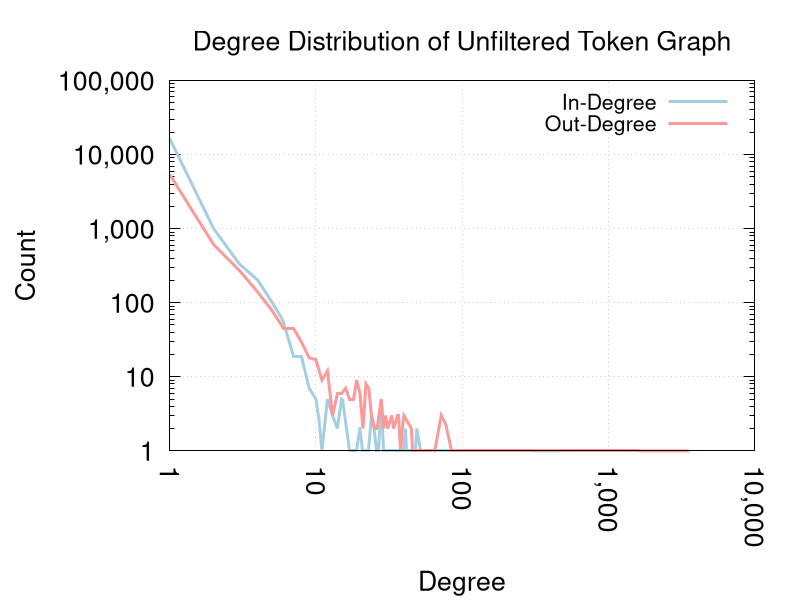
\includegraphics[width=\columnwidth]{img/degree-distributions/unfiltered-token-graph-degrees.png}}
  \caption{The in- and out-degree distributions for the unfiltered
    token graph show an inverse relationship between the degree of a
    vertex and the number of vertices with that degree in the graph.
    There are a small number of vertices with high degree and a large
    number of vertices with low
    degree.}\label{fig:unfiltered-token-graph-degrees}
\end{figure}

\begin{figure}
  \centerline{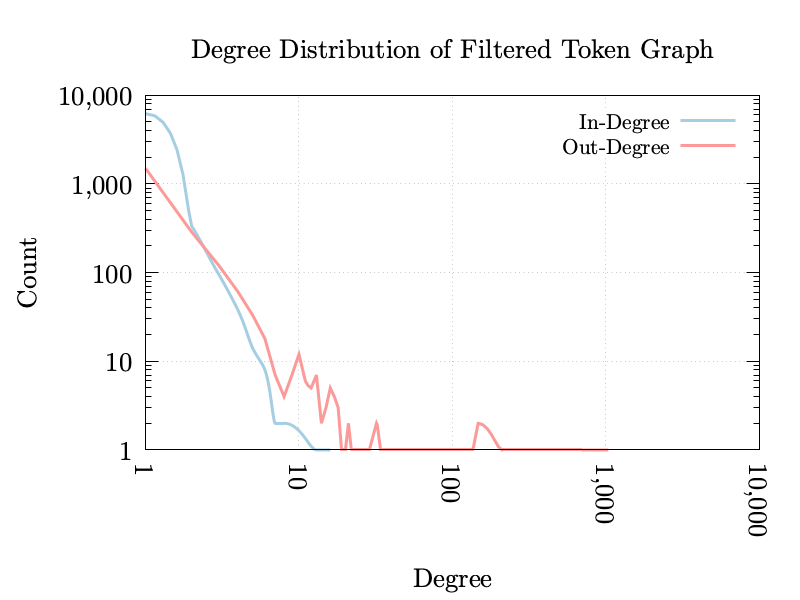
\includegraphics[width=\columnwidth]{img/degree-distributions/filtered-token-graph-degrees.png}}
  \caption{The in- and out-degree distributions for the filtered token
    graph show a similar inverse relationship as in
    Fig.~\ref{fig:unfiltered-token-graph-degrees}.}\label{fig:filtered-token-graph-degrees}
\end{figure}

\begin{figure}
  \centerline{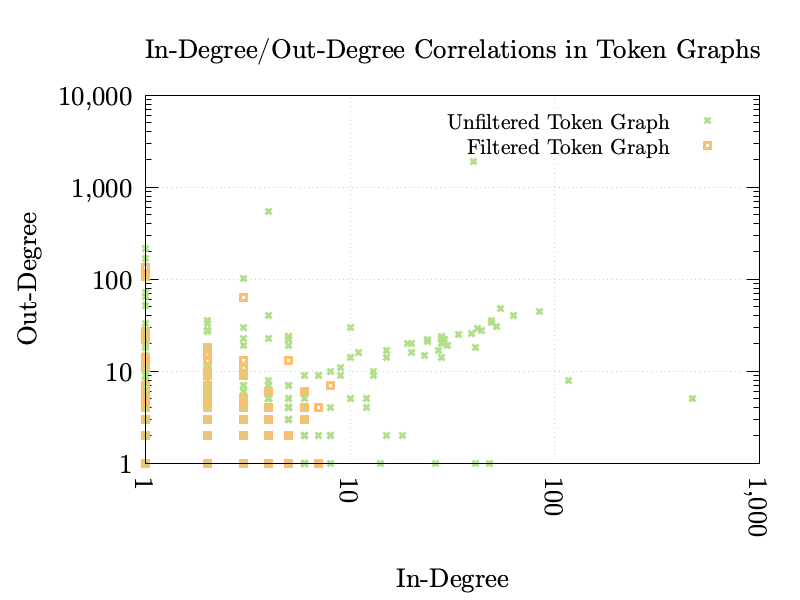
\includegraphics[width=\columnwidth]{img/degree-distributions/token-graph-in-out-degrees.png}}
  \caption{In both the unfiltered and filtered token graphs, there are
    vertices with low in-degree and low out-degree, high in-degree and
    low out-degree, low in-degree and high out-indegree, and high
    in-degree and high out-degree.  We consider examples of each in
    Sect.~\ref{sec:analysis-degree-distribution}.}\label{fig:token-graph-in-out-degrees}
\end{figure}

\subsection{Cyclic Structure}\label{sec:analysis-cyclic-structure}

\subsection{Component Structure}\label{sec:analysis-component-structure}
